\documentclass[aspectratio=169,xcolor={dvipsnames}]{beamer}

% XeLaTeX packages
\usepackage{fontspec}
\usepackage{xcolor}
\usepackage{tikz}
\usetikzlibrary{positioning}
\usepackage{booktabs}
\usepackage{amsmath}
\usepackage{amsthm}
\usepackage{caption}
\usepackage{graphicx}
\usepackage{listings}
\usepackage{biblatex}

% Bibliography
\addbibresource{references_new.bib}

% Modern theme configuration
\usetheme{Boadilla}
\usecolortheme{default}

% Define complementary palette based on VU Blue
\definecolor{VUBlue}{HTML}{0057B7}
\definecolor{Endeavour}{HTML}{0754AA}
\definecolor{AbsoluteZero}{HTML}{055AB9}
\definecolor{ScienceBlue}{HTML}{0360C8}
\definecolor{RustyNail}{HTML}{8E4F09}
\definecolor{RichGold}{HTML}{9C5608}
\definecolor{LightGray}{HTML}{E8E9EA}
\definecolor{Charcoal}{HTML}{222831}

% Set theme colors
\setbeamercolor{frametitle}{bg=VUBlue, fg=white}
\setbeamercolor{title}{fg=VUBlue}
\setbeamercolor{structure}{fg=ScienceBlue}
\setbeamercolor{alerted text}{fg=RustyNail}
\setbeamercolor{block title}{bg=AbsoluteZero, fg=white}
\setbeamercolor{block body}{bg=LightGray, fg=Charcoal}
\setbeamercolor{alertblock title}{bg=RustyNail, fg=white}
\setbeamercolor{alertblock body}{bg=LightGray, fg=Charcoal}

% Font settings
\setmainfont{Liberation Sans}
\setsansfont{Liberation Sans}
\setmonofont{Liberation Mono}[Scale=0.9]

% Custom commands
\newcommand{\highlight}[1]{\textcolor{RustyNail}{\textbf{#1}}}
\newcommand{\code}[1]{\texttt{\small #1}}
\newcommand{\phase}[1]{\textcolor{ScienceBlue}{\textbf{Phase #1}}}

% Configure listings
\lstset{
  basicstyle=\ttfamily\footnotesize,
  backgroundcolor=\color{LightGray},
  frame=single,
  breaklines=true
}

% Title page info
\title{Privacy-Preserving Synthetic Trajectory Generation}
\subtitle{An Integrated DiffTraj-LM-TAD Framework for Taxi Route Anomaly Detection}
\author{Mateusz Kędzia}
\institute{MSc Artificial Intelligence \\ Vrije Universiteit Amsterdam}
\date{Thesis Progress Presentation -- July 2025}

% Custom title page
\defbeamertemplate*{title page}{customized}[1][]
{%
  \vbox{}
  \vfill
  \begingroup
    \centering
    \begin{beamercolorbox}[sep=8pt,center,#1]{title}
      \usebeamerfont{title}\inserttitle\par%
      \ifx\insertsubtitle\@empty%
      \else%
        \vskip0.25em%
        {\usebeamerfont{subtitle}\usebeamercolor[fg]{subtitle}\insertsubtitle\par}%
      \fi%     
    \end{beamercolorbox}%
    \vskip1em\par
    \begin{beamercolorbox}[sep=8pt,center,#1]{author}
      \usebeamerfont{author}\insertauthor
    \end{beamercolorbox}
    \begin{beamercolorbox}[sep=8pt,center,#1]{institute}
      \usebeamerfont{institute}\insertinstitute
    \end{beamercolorbox}
    \begin{beamercolorbox}[sep=8pt,center,#1]{date}
      \usebeamerfont{date}\insertdate
    \end{beamercolorbox}\vskip0.5em
  \endgroup
  \vfill
}

\begin{document}

% --- Title Slide ---
\begin{frame}[plain]
  \vspace{1.5cm}
  \centering
  {\usebeamerfont{title}\color{VUBlue}\Huge\textbf{Privacy-Preserving Synthetic Trajectory Generation}}
  
  \vspace{0.5em}
  {\usebeamerfont{subtitle}\color{RichGold}\Large An Integrated DiffTraj-LM-TAD Framework}
  
  \vspace{1.5em}
  {\usebeamerfont{author}\large Mateusz Kędzia}
  
  \vspace{0.5em}
  {\usebeamerfont{institute}\normalsize MSc Artificial Intelligence \\ Vrije Universiteit Amsterdam}
  
  \vspace{1em}
  {\usebeamerfont{date}\small Thesis Progress Presentation -- July 2025}
\end{frame}

% --- Problem & Solution ---
\begin{frame}{The Challenge}
  \begin{alertblock}{Privacy vs. Utility Paradox}
    \centering
    \Large Traditional privacy methods degrade spatio-temporal patterns needed for anomaly detection \cite{buchholzSystematisationKnowledgeTrajectory2024}
  \end{alertblock}
  
  \vspace{1em}
  \begin{block}{Our Solution: Bootstrap Approach}
    \centering
    \textbf{Privacy by Design} + \textbf{High Utility} + \textbf{Anomaly Detection Ready}
    
    \vspace{0.5em}
    \textit{``Bootstraps anomaly generation without pre-labeled dataset''}
  \end{block}
\end{frame}

% --- Core Process Overview ---
\begin{frame}{3-Phase Bootstrap Framework}
  \begin{center}
    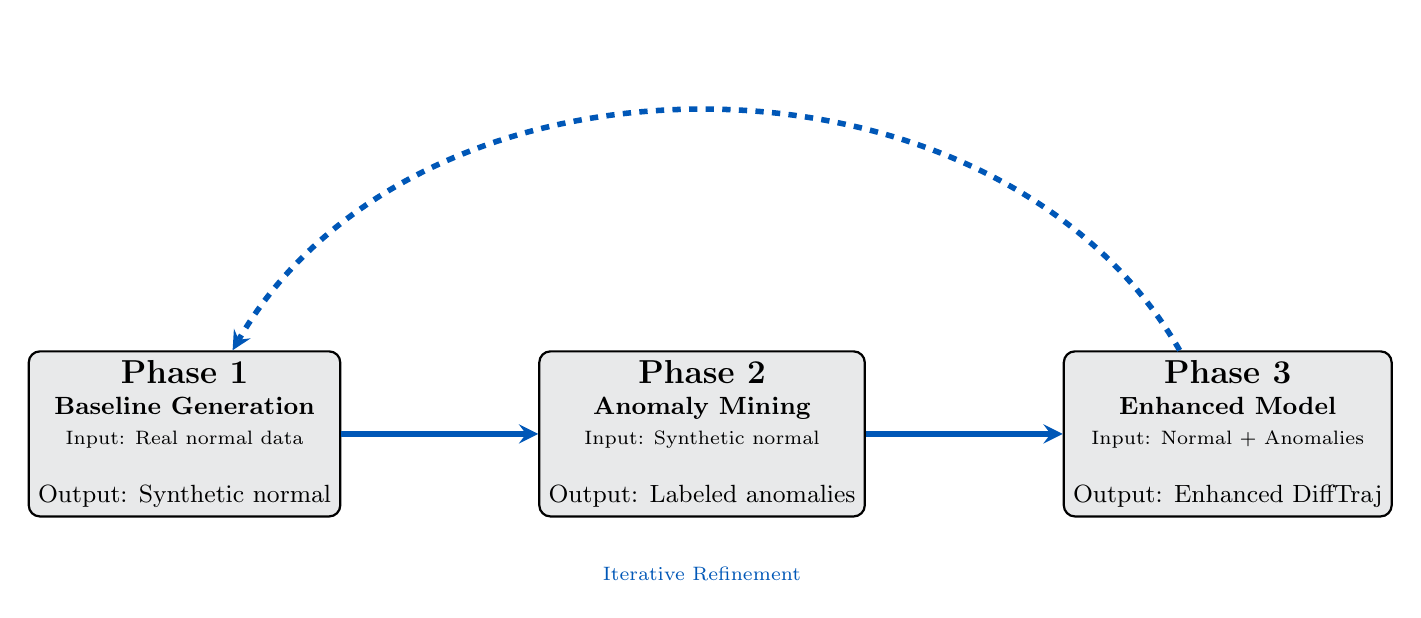
\begin{tikzpicture}[
      node distance=2.5cm,
      every node/.style={align=center, font=\small},
      box/.style={draw, fill=LightGray, rounded corners, minimum width=3.5cm, minimum height=2cm, thick},
      arrow/.style={thick, VUBlue, ->, >=stealth, line width=2pt}
    ]
      
      % Phase boxes
      \node[box] (phase1) {\textbf{\large Phase 1}\\\textbf{Baseline Generation}\\\vspace{0.3cm}\scriptsize Input: Real normal data\\Output: Synthetic normal};
      
      \node[box, right=of phase1] (phase2) {\textbf{\large Phase 2}\\\textbf{Anomaly Mining}\\\vspace{0.3cm}\scriptsize Input: Synthetic normal\\Output: Labeled anomalies};
      
      \node[box, right=of phase2] (phase3) {\textbf{\large Phase 3}\\\textbf{Enhanced Model}\\\vspace{0.3cm}\scriptsize Input: Normal + Anomalies\\Output: Enhanced DiffTraj};
      
      % Arrows
      \draw[arrow] (phase1) -- (phase2);
      \draw[arrow] (phase2) -- (phase3);
      
      % Feedback loop
      \draw[arrow, dashed] (phase3) to[bend right=60] (phase1);
      \node[below=0.5cm of phase2, font=\scriptsize\color{VUBlue}] {Iterative Refinement};
      
    \end{tikzpicture}
  \end{center}
\end{frame}

% --- Phase 1 Detail ---
\begin{frame}{Phase 1: Baseline Generation}
  \begin{center}
    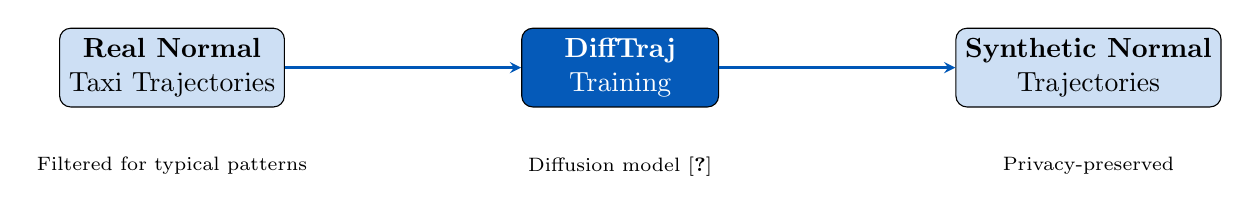
\begin{tikzpicture}[
      node distance=3cm,
      every node/.style={align=center},
      data/.style={draw, fill=ScienceBlue!20, rounded corners, minimum width=2cm, minimum height=1cm},
      process/.style={draw, fill=AbsoluteZero, text=white, rounded corners, minimum width=2.5cm, minimum height=1cm},
      arrow/.style={thick, VUBlue, ->, >=stealth}
    ]
      
      \node[data] (input) {\textbf{Real Normal}\\Taxi Trajectories};
      \node[process, right=of input] (difftraj) {\textbf{DiffTraj}\\Training};
      \node[data, right=of difftraj] (output) {\textbf{Synthetic Normal}\\Trajectories};
      
      \draw[arrow] (input) -- (difftraj);
      \draw[arrow] (difftraj) -- (output);
      
      % Labels
      \node[below=0.5cm of input, font=\scriptsize] {Filtered for typical patterns};
      \node[below=0.5cm of difftraj, font=\scriptsize] {Diffusion model \cite{zhuDiffTrajGeneratingGPS2023}};
      \node[below=0.5cm of output, font=\scriptsize] {Privacy-preserved};
      
    \end{tikzpicture}
  \end{center}
  
  \vspace{1em}
  \begin{block}{Key Innovation: Differential Privacy}
    DP-SGD with privacy budget $\varepsilon = 2.0$ ensures bounded influence of individual trajectories
  \end{block}
\end{frame}

% --- Phase 2 Detail ---
\begin{frame}{Phase 2: Anomaly Mining}
  \begin{center}
    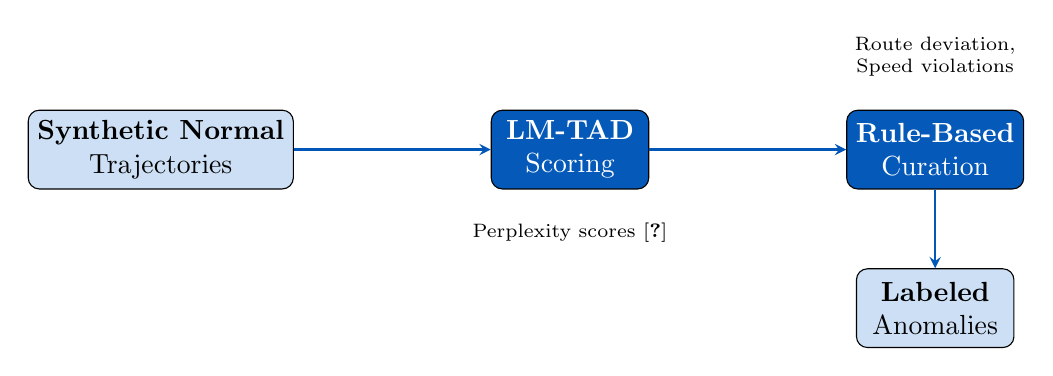
\begin{tikzpicture}[
      node distance=2.5cm,
      every node/.style={align=center},
      data/.style={draw, fill=ScienceBlue!20, rounded corners, minimum width=2cm, minimum height=1cm},
      process/.style={draw, fill=AbsoluteZero, text=white, rounded corners, minimum width=2cm, minimum height=1cm},
      arrow/.style={thick, VUBlue, ->, >=stealth}
    ]
      
      \node[data] (input) {\textbf{Synthetic Normal}\\Trajectories};
      \node[process, right=of input] (lmtad) {\textbf{LM-TAD}\\Scoring};
      \node[process, right=of lmtad] (rules) {\textbf{Rule-Based}\\Curation};
      \node[data, below=1cm of rules] (output) {\textbf{Labeled}\\Anomalies};
      
      \draw[arrow] (input) -- (lmtad);
      \draw[arrow] (lmtad) -- (rules);
      \draw[arrow] (rules) -- (output);
      
      % Labels
      \node[below=0.3cm of lmtad, font=\scriptsize] {Perplexity scores \cite{mbuyaTrajectoryAnomalyDetection2024}};
      \node[above=0.3cm of rules, font=\scriptsize] {Route deviation,\\Speed violations};
      
    \end{tikzpicture}
  \end{center}
  
  \vspace{1em}
  \begin{block}{Unsupervised Detection}
    LM-TAD treats trajectories as token sequences, identifying anomalies through language modeling perplexity
  \end{block}
\end{frame}

% --- Phase 3 Detail ---
\begin{frame}{Phase 3: Enhanced Model}
  \begin{center}
    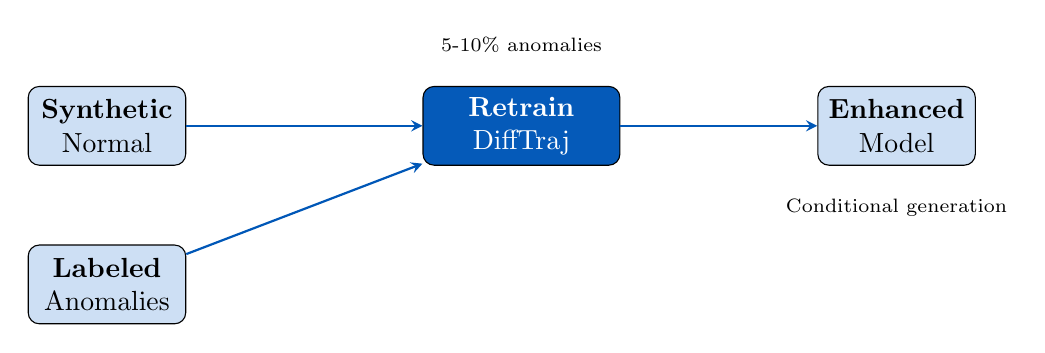
\begin{tikzpicture}[
      node distance=2.5cm,
      every node/.style={align=center},
      data/.style={draw, fill=ScienceBlue!20, rounded corners, minimum width=2cm, minimum height=1cm},
      process/.style={draw, fill=AbsoluteZero, text=white, rounded corners, minimum width=2.5cm, minimum height=1cm},
      arrow/.style={thick, VUBlue, ->, >=stealth}
    ]
      
      \node[data] (normal) {\textbf{Synthetic}\\Normal};
      \node[data, below=1cm of normal] (anomaly) {\textbf{Labeled}\\Anomalies};
      \node[process, right=3cm of normal] (retrain) {\textbf{Retrain}\\DiffTraj};
      \node[data, right=of retrain] (output) {\textbf{Enhanced}\\Model};
      
      \draw[arrow] (normal) -- (retrain);
      \draw[arrow] (anomaly) -- (retrain);
      \draw[arrow] (retrain) -- (output);
      
      % Merge indicator
      \node[above=0.3cm of retrain, font=\scriptsize] {5-10\% anomalies};
      \node[below=0.3cm of output, font=\scriptsize] {Conditional generation};
      
    \end{tikzpicture}
  \end{center}
  
  \vspace{1em}
  \begin{block}{Iterative Improvement}
    Enhanced model generates both normal and anomalous trajectories with improved diversity and realism
  \end{block}
\end{frame}

% --- Privacy Framework ---
\begin{frame}{Privacy-by-Design Framework}
  \begin{center}
    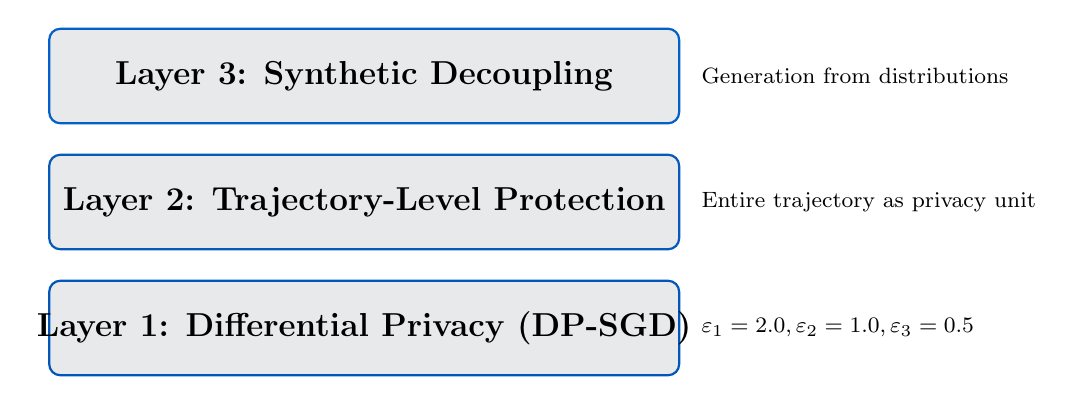
\begin{tikzpicture}[scale=0.8]
      % Three layers
      \draw[fill=LightGray, draw=VUBlue, thick, rounded corners] (0,0) rectangle (10,1.5);
      \node at (5,0.75) {\large\textbf{Layer 1: Differential Privacy (DP-SGD)}};
      
      \draw[fill=LightGray, draw=AbsoluteZero, thick, rounded corners] (0,2) rectangle (10,3.5);
      \node at (5,2.75) {\large\textbf{Layer 2: Trajectory-Level Protection}};
      
      \draw[fill=LightGray, draw=ScienceBlue, thick, rounded corners] (0,4) rectangle (10,5.5);
      \node at (5,4.75) {\large\textbf{Layer 3: Synthetic Decoupling}};
      
      % Privacy budgets
      \node[right] at (10.2,0.75) {\footnotesize $\varepsilon_1=2.0, \varepsilon_2=1.0, \varepsilon_3=0.5$};
      \node[right] at (10.2,2.75) {\footnotesize Entire trajectory as privacy unit};
      \node[right] at (10.2,4.75) {\footnotesize Generation from distributions};
      
    \end{tikzpicture}
  \end{center}
  
  \vspace{1em}
  \begin{alertblock}{}
    \centering
    Multi-layer defense prevents both membership inference and reconstruction attacks \cite{buchholzSystematisationKnowledgeTrajectory2024}
  \end{alertblock}
\end{frame}

% --- Evaluation & Results ---
\begin{frame}{Evaluation Framework}
  \begin{columns}[T,onlytextwidth]
    \begin{column}{0.48\textwidth}
      \begin{block}{Datasets}
        \begin{itemize}
          \item \textbf{Beijing}: Primary development
          \item \textbf{Chengdu}: Cross-city validation
          \item \textbf{Xi'an}: Urban diversity testing
        \end{itemize}
      \end{block}
    \end{column}
    \hspace{0.04\textwidth}
    \begin{column}{0.48\textwidth}
      \begin{block}{Metrics}
        \begin{itemize}
          \item \textbf{Detection}: Precision, Recall, F1
          \item \textbf{Quality}: SDMetrics suite
          \item \textbf{Privacy}: Attack resistance
        \end{itemize}
      \end{block}
    \end{column}
  \end{columns}
\end{frame}

% --- Key Contributions ---
\begin{frame}{Key Contributions}
  \begin{block}{}
    \begin{enumerate}
      \item \textbf{First integrated DiffTraj + LM-TAD framework} for privacy-preserving trajectory generation
      \item \textbf{Bootstrap methodology} that generates anomalies without pre-labeled datasets
      \item \textbf{Multi-layer privacy protection} preserving spatio-temporal patterns for anomaly detection
    \end{enumerate}
  \end{block}
  
  \vspace{1em}
  \begin{alertblock}{Current Status}
    \centering
    Phase 1 implementation in progress | Phases 2-3 planned for completion by thesis defense
  \end{alertblock}
\end{frame}

% --- Thank You ---
\begin{frame}[plain]
  \centering
  \Huge \textbf{Thank You}
  
  \vspace{0.5em}
  \Large \textbf{Questions \& Discussion}
  
  \vspace{2em}
  \begin{block}{}
    \centering
    \textbf{Privacy-Preserving} | \textbf{Bootstrap Approach} | \textbf{Real-World Applications}
  \end{block}
\end{frame}

% --- References ---
\begin{frame}[allowframebreaks]{References}
  \begin{block}{}
    \footnotesize
    \printbibliography[heading=none]
  \end{block}
\end{frame}

\end{document} 